\section{Failures}
\label{s:failures}
We propose several natural approaches to achieve $T$-fault tolerance, both for local and central machines, where the different approaches differ in which aspect of the system is sacrificed to achieve such a fault tolerant system. For simplicity, we only discuss failures in the non-dynamic case where we are trying to build a summary from a fixed ground set of elements. Note that the issue of failure is not addressed in \cite{mirzasoleiman2013distributed} where the non-dynamic algorithm is presented.

\subsection{Failures on local machines}

The first technique to achieve $T$-fault tolerance on local machines is very simple. The central machine waits until it receives $m -T$ local solutions from $m-T$ local machines before computing a central solution. It is easy to see that the central solution will be built unless there are more than $T$ local machines that fail. The tradeoff here is between achieving a higher fault tolerance system and the \textit{approximation ratio} since the central machine has access to less elements as if it waited for all local solutions.

\begin{figure}
    \centering
    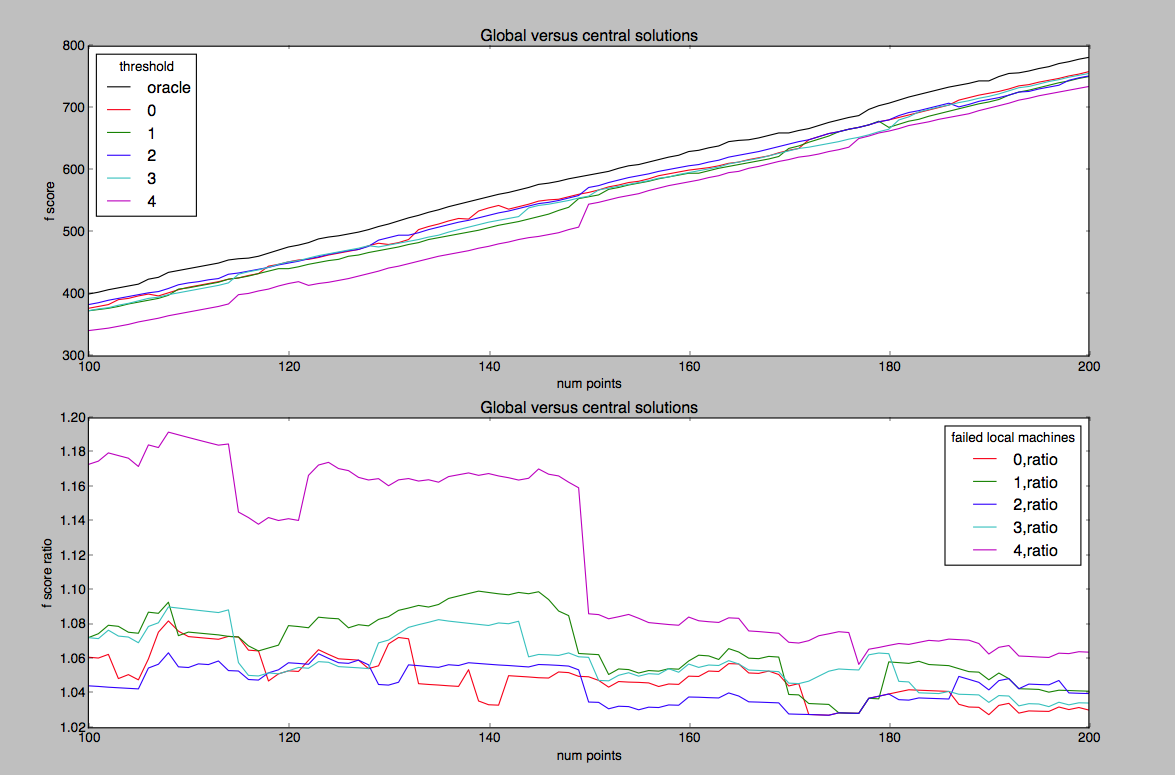
\includegraphics[width=\linewidth]{failplot}
    \caption{Robustness to local machine failure}
     \label{fig:fail}
\end{figure}

Experimentally, we can demonstrate this fault tolerance. The central process in our system recalculates every time it receives an update and does not in fact wait to receive a full set of representatives before it selects from them. Having local processes fail, the central process is just left with fewer or less up-to-date candidates to choose from. Figure \ref{fig:fail} shows the effect on the central process score and approximation ration of local machine failure. This plot shows the results of a simulation with 100 initial data points, 100 insertions, and 5 local files. Different colors correspond to different numbers of local machines that never communicate with the central server, so e.g. the pink line corresponds to a run in which the solution is only affected by 1/3 of the data (1/6 in the central process and 1/6 in the lone functioning local process). We see that even for a very small dataset, local failure degrades performance fairly gracefully.

The second approach maintains $T+1$ replications of each element from the ground set $N$ on $T+1$ distinct local machines and, similarly as with the previous technique, the central machine waits to receive $m-T$ local solutions. Again, it is easy that this system is $T$-fault tolerant. The main difference with this approach is that instead of sacrificing the approximation ratio, the \textit{memory per local machine} 
needed increases. The approximation ratio is not sacrificed anymore since for each element $e \in N$, the central machine will receive a solution from at least one local machine containing $e$.

\subsection{Failures on central machine}

Regarding failures on central machine, a natural approach is to run a leader election algorithm among the local machines and to rerun the non-dynamic algorithm if the central machine fails. The drawback of this approach is the \textit{runtime} since the algorithm needs to rerun every time the central machine fails. To avoid sacrificing the runtime, an alternative approach is to have $T+1$ central machines instead of one. The sacrifice here is the \textit{communication complexity} since the local machines must send their local solutions to $T+1$ different machines instead of one.

